\documentclass[main]{subfiles}
\begin{document}

%@@@@@@@@@@@@@@@@@@@@@@@@@@@@@@
% Main Topics: Action Potential 18.10.2018
% Lecturer: Valerio Mante
% author: Vanessa Leite - base document from benelot/eth-intro-to-neuroinformatics-summary

\section{Action Potential}
\begin{itemize}[noitemsep,nolistsep]
	\item Refraction period ensures maximum frequency.
	\item Action potential is about $1$ to $10\,m/s$ fast.
	\item It would take 100 years to go through all axons of the human brain in a serial fashion.
\end{itemize}
\subsection{Equilibrium voltage}
\begin{itemize}[noitemsep,nolistsep]
	\item When $I_m = 0$ and $\frac{dv}{dt}=0$ then
	\item $V=\frac{g_KE_K+g_{Na}E_{Na}+g_{Cl}E_{Cl}}{g_K+g_{Na}+g_{Cl}}$
	\item $I_m = I_{cap}+I_K+I_{Na}+I_{L}$
\end{itemize}

\subsection{Voltage clamp experiment}
\begin{itemize}[noitemsep,nolistsep]
	\item Command voltage is set by the experimenter, the feedback circuit holds the voltage constant.
	\item The voltage clamp allows the membrane voltage to be manipulated independently of ionic currents, allowing the current-voltage relationships of membrane channels to be studied.
	\item With negative feedback circuit, the $Na^+$ current is auto-catalytic. An increase in the voltage increases conductance, which increases the $Na^+$ current, which increases the voltage again.
	\item Voltage and time dependent conductances for $g_{Na}, g_{K}$:
	\subitem $g_{Na}$ increases quickly, but then inactivation kicks in and it decreases again.
	\subitem $g_K$ increases more slowly, and only decreases once the voltage has decreased.
	\item The threshold for action potential initiation is where the inward $Na^+$ current exactly balances the outward $K^+$ current.
\end{itemize}

\begin{figure}[H]
	\centering
	\begin{subfigure}[b]{0.5\textwidth}
    	\centering
		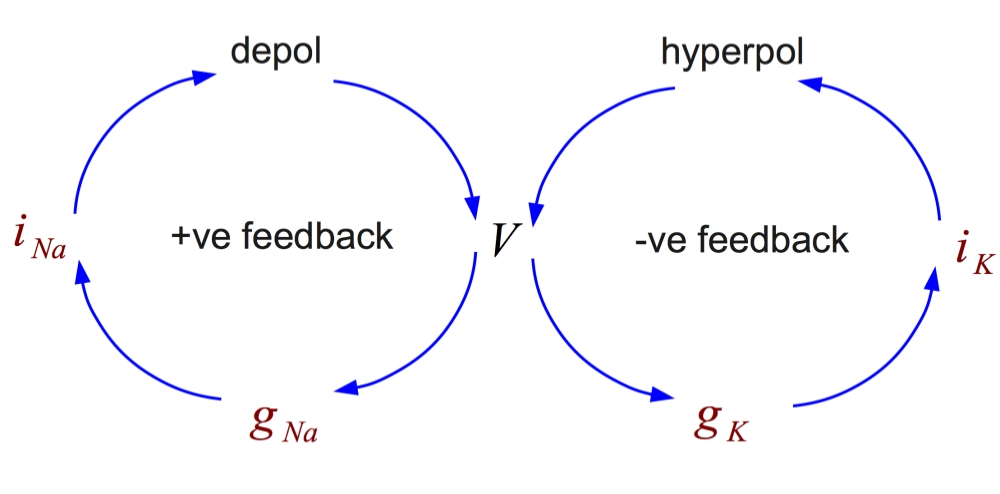
\includegraphics[width=\textwidth]{5_7.jpg}
	\end{subfigure}%
	~
	\begin{subfigure}[b]{0.5\textwidth}
		\centering
		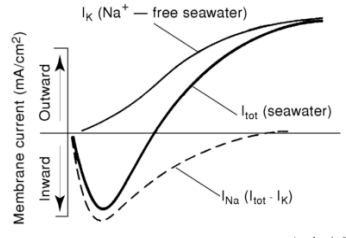
\includegraphics[width=\textwidth]{voltage_clamp_01.png}
	\end{subfigure}
\end{figure}

\begin{figure}[H]
	\centering
	\begin{subfigure}[b]{0.65\textwidth}
    	\centering
		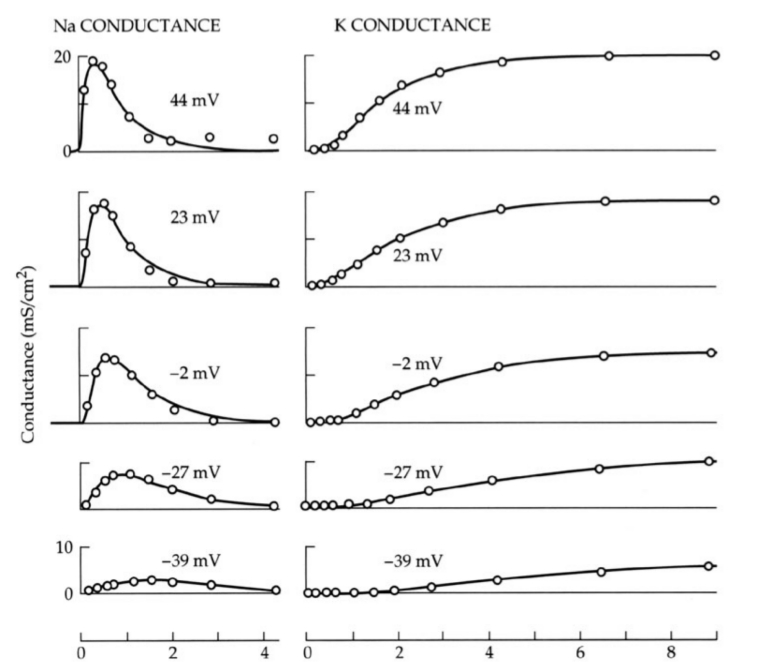
\includegraphics[width=\textwidth]{5_4.jpg}
	\end{subfigure}%
	~
	\begin{subfigure}[b]{0.35\textwidth}
		\centering
		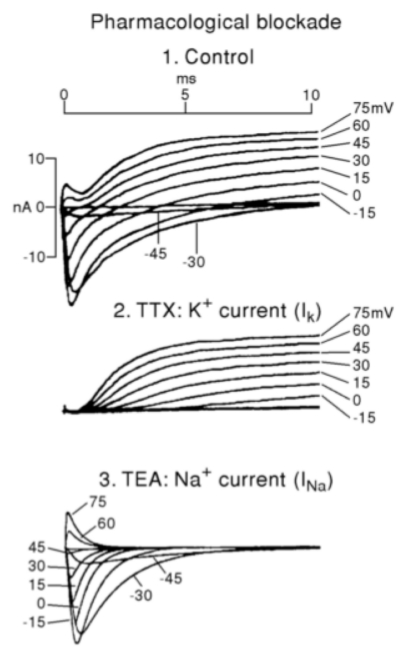
\includegraphics[width=\textwidth]{5_4_2.jpg}
	\end{subfigure}
\end{figure}



\end{document}
